\documentclass[12pt,a4paper]{article}
\usepackage[a4paper,margin=1in]{geometry}
\usepackage{listings}
\usepackage{xcolor}
\usepackage{hyperref}
\usepackage{tikz}
\usetikzlibrary{arrows,shapes,positioning}
\usepackage{amsmath}
\hypersetup{
    colorlinks=true,
    linkcolor=blue,
    urlcolor=blue
}


% Define color palette
\definecolor{codebg}{HTML}{F8F8F8}
\definecolor{codeborder}{HTML}{DDDDDD}
\definecolor{keywordcolor}{HTML}{005CC5}
\definecolor{stringcolor}{HTML}{032F62}
\definecolor{commentcolor}{HTML}{6A737D}
\definecolor{typecolor}{HTML}{D73A49}
\definecolor{numbercolor}{HTML}{005CC5}
% --------- Refined Assembly Code Listing Style ---------
\lstdefinestyle{asm}{
    language=[x86masm]Assembler,
    backgroundcolor=\color{codebg},
    basicstyle=\linespread{1.05}\ttfamily\footnotesize,
    numbers=left,
    numberstyle=\tiny\color{gray},
    numbersep=10pt,
    frame=single,
    rulecolor=\color{codeborder},
    tabsize=4,
    showstringspaces=false,
    breaklines=true,
    keywordstyle=\color{keywordcolor}\bfseries,
    stringstyle=\color{stringcolor},
    commentstyle=\color{commentcolor}\itshape,
    identifierstyle=\color{black},
    emphstyle=\color{typecolor}\bfseries,
    morekeywords={
        mov,push,pop,call,ret,int,iret,
        cli,sti,hlt,jmp,jz,jnz,je,jne,jg,jl,jge,jle,
        cmp,inc,dec,add,sub,mul,div,and,or,xor,not,
        in,out,shl,shr,test,nop,org,db,dd,dw,times
    },
    literate=
        *{0}{{{\color{numbercolor}0}}}{1}
         {1}{{{\color{numbercolor}1}}}{1}
         {2}{{{\color{numbercolor}2}}}{1}
         {3}{{{\color{numbercolor}3}}}{1}
         {4}{{{\color{numbercolor}4}}}{1}
         {5}{{{\color{numbercolor}5}}}{1}
         {6}{{{\color{numbercolor}6}}}{1}
         {7}{{{\color{numbercolor}7}}}{1}
         {8}{{{\color{numbercolor}8}}}{1}
         {9}{{{\color{numbercolor}9}}}{1},
    captionpos=b,
    framexleftmargin=14pt,
    framexrightmargin=8pt,
    framextopmargin=4pt,
    framexbottommargin=4pt,
    frameround=tttt,
    xleftmargin=1.5em,
    xrightmargin=0.5em,
    aboveskip=1em,
    belowskip=1em,
    backgroundcolor=\color{codebg},
    rulesepcolor=\color{codeborder},
    rulecolor=\color{codeborder}
}

\lstdefinestyle{c++}{
    language=C,
    backgroundcolor=\color{codebg},
    basicstyle=\linespread{1.05}\ttfamily\footnotesize,
    numbers=left,
    numberstyle=\tiny\color{gray},
    numbersep=10pt,
    frame=single,
    rulecolor=\color{codeborder},
    tabsize=4,
    showstringspaces=false,
    breaklines=true,
    keywordstyle=\color{keywordcolor}\bfseries,
    stringstyle=\color{stringcolor},
    commentstyle=\color{commentcolor}\itshape,
    identifierstyle=\color{black},
    emphstyle=\color{typecolor}\bfseries,
    morekeywords={uint8_t,uint16_t,uint32_t,ISR,IRQ,stackframe},
    literate=
        *{0}{{{\color{numbercolor}0}}}{1}
         {1}{{{\color{numbercolor}1}}}{1}
         {2}{{{\color{numbercolor}2}}}{1}
         {3}{{{\color{numbercolor}3}}}{1}
         {4}{{{\color{numbercolor}4}}}{1}
         {5}{{{\color{numbercolor}5}}}{1}
         {6}{{{\color{numbercolor}6}}}{1}
         {7}{{{\color{numbercolor}7}}}{1}
         {8}{{{\color{numbercolor}8}}}{1}
         {9}{{{\color{numbercolor}9}}}{1},
    captionpos=b,
    framexleftmargin=14pt,
    framexrightmargin=8pt,
    framextopmargin=4pt,
    framexbottommargin=4pt,
    frameround=tttt,
    xleftmargin=1.5em,
    xrightmargin=0.5em,
    aboveskip=1em,
    belowskip=1em,
    backgroundcolor=\color{codebg},
    rulesepcolor=\color{codeborder},
    rulecolor=\color{codeborder}
}


\title{Intel Kernel Programming: A Guide to Intel's Security Mechanisms and Multitasking}
\author{Marco Paviotti}
\date{November 2025}

\begin{document}
\maketitle
\tableofcontents
\newpage

\section{Introduction}
Modern x86 operating systems rely on the transition from real mode to protected
mode to take advantage of 32-bit addressing, hardware-enforced privilege levels,
and memory protection~\cite{tanenbaum2015modern,stallings2021operating,osdevwiki}.

When a modern x86 processor powers on, it begins execution in \textit{real
mode}, a legacy environment compatible with the 8086 CPU. In real mode, memory
addressing is limited to 1 MB, there is no enforced protection, and the CPU
treats all instructions and I/O operations as fully trusted.

This manual guides you from real mode to protected mode, explaining how the CPU
enforces privilege levels using rings, how segmentation and paging work, and how
multitasking can be implemented via interrupts. All examples are in NASM and can
be tested on macOS using Bochs or QEMU.

\section{The BIOS Boot Phase}
When a computer is powered on, the processor begins executing firmware
instructions stored in ROM. This firmware, traditionally called the
\textbf{BIOS} (Basic Input/Output System), performs several key tasks before any
operating system code runs. It initializes basic hardware, performs a Power-On
Self Test (POST) to verify that essential components such as memory, keyboard,
and display are working, and then begins searching for a bootable device
according to a configured boot order (for example, floppy disk, hard drive, or
CD-ROM).

Once a bootable device is found, the BIOS loads exactly \textbf{one sector of
data} from that device into memory. A sector on a floppy or hard disk is always
\textbf{512 bytes} in size. The BIOS reads this single 512-byte block---known as
the \textbf{boot sector}---into memory at the address \texttt{0x7C00}. After
copying those 512 bytes, the BIOS transfers control to that address, effectively
beginning execution of the bootloader code contained in the boot sector.

The BIOS uses a very simple validation step to determine whether the sector it
has loaded is indeed a valid boot sector. At the end of the 512-byte block, the
last two bytes (offsets \texttt{0x1FE} and \texttt{0x1FF}) must contain the
values \texttt{0x55} and \texttt{0xAA} respectively. This two-byte sequence is
known as the \textbf{boot signature}. If the signature is missing or incorrect,
the BIOS assumes the device is not bootable and continues scanning the next
device in its boot order.

Therefore, the layout of the boot sector is fixed by convention: the first 510 bytes (\texttt{0x000}--\texttt{0x1FD}) contain the executable bootloader code, and the final two bytes (\texttt{0x1FE}--\texttt{0x1FF}) contain the boot signature. A minimal bootloader, such as one written in NASM, fits entirely into these 510 bytes. Its primary responsibility is to prepare the CPU state (set up segment registers, stack, and possibly the video mode), and then to load additional sectors---the second-stage loader or kernel---from disk into memory.

The BIOS itself has no knowledge of the size or structure of the operating system to be loaded. It performs only this small but critical action: reading one sector and jumping to it. Everything that follows, including reading more data, initializing protected mode, and setting up paging, must be performed by the bootloader. The entire early boot sequence can be summarized as follows:

\begin{center}
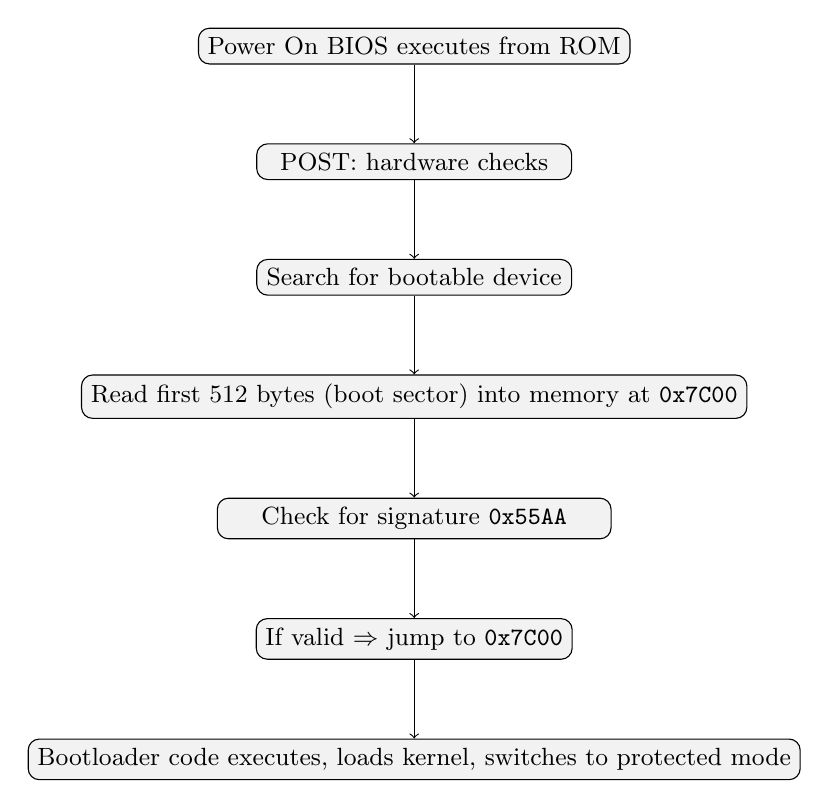
\begin{tikzpicture}[node distance=1cm, every node/.style={font=\small}]
\node (start) [draw, rounded corners, align=center, fill=gray!10, minimum width=4cm] {Power On  BIOS executes from ROM};
\node (post) [draw, below=of start, rounded corners, fill=gray!10, minimum width=4cm] {POST: hardware checks};
\node (search) [draw, below=of post, rounded corners, fill=gray!10, minimum width=4cm] {Search for bootable device};
\node (read) [draw, below=of search, rounded corners, fill=gray!10, minimum width=5cm] {Read first 512 bytes (boot sector) into memory at \texttt{0x7C00}};
\node (check) [draw, below=of read, rounded corners, fill=gray!10, minimum width=5cm] {Check for signature \texttt{0x55AA}};
\node (jump) [draw, below=of check, rounded corners, fill=gray!10, minimum width=4cm] {If valid $\Rightarrow$ jump to \texttt{0x7C00}};
\node (boot) [draw, below=of jump, rounded corners, fill=gray!10, minimum width=6cm] {Bootloader code executes, loads kernel, switches to protected mode};

\draw[->] (start) -- (post);
\draw[->] (post) -- (search);
\draw[->] (search) -- (read);
\draw[->] (read) -- (check);
\draw[->] (check) -- (jump);
\draw[->] (jump) -- (boot);
\end{tikzpicture}
\end{center}

In summary, the BIOS always reads exactly one 512-byte sector from the boot
device into address \texttt{0x7C00} and checks for the signature
\texttt{0x55AA}. This tiny amount of code is what begins the entire operating
system loading process.

\section{Real Mode}
Before the Intel 80286, the architecture used 16-bit registers, which meant that
memory addresses were also 16-bit. This allowed the processor to directly access
only 64 KB of memory. However, with a clever technique, the x86 processors could
address up to 1 MB by using a second register called a \textit{selector} which
selects the block and another 16-bit register called \textit{offset}.
Essentially, memory was divided into 64 KB blocks, which could be addressed
using the normal registers, while the selector register chose which block was
active. In real mode, the CPU calculates physical memory addresses using 16-bit
segment registers and 16-bit offsets according to the formula:
\[
  \mathrm{Physical\ Address} = (\mathrm{Segment Selector} \times 16) + \mathrm{Offset}
\]
The maximum physical address occurs when both the segment and offset registers are at their maximum values:
\[
\mathrm{Max Address} = (\mathrm{0xFFFF} \times 16) + \mathrm{0xFFFF}
\]
Calculating step by step, \(\mathrm{0xFFFF} = 65535\) in decimal. Multiplying by
16 gives \(65535 \times 16 = 1048560\). Adding the maximum offset
\(\mathrm{0xFFFF} = 65535\) gives a total of \(1048560 + 65535 = 1114095\),
which is \(\mathrm{0x10FFFF}\) in hexadecimal.

The main segment registers are CS, DS, SS, ES, and, on modern processors, FS and
GS. The CS register, or Code Segment, points to the segment containing the
currently executing instructions, and it is paired with the Instruction Pointer
(IP) to determine which instruction to fetch. For example, when executing an
instruction, the processor would calculate the physical address as:
\[
\text{Physical Address} = \text{CS} \times 16 + \text{IP}
\]
where CS is the Code Segment selector and IP is the Instruction Pointer. This
produces a 20-bit physical address, which is then placed on the address bus.

The DS register, or Data Segment, is the default segment used for data accesses
such as loading or storing variables; general-purpose registers like BX, SI, DI,
and BP are typically used as offsets within DS. The SS register, or Stack
Segment, points to the stack, with SP (Stack Pointer) and BP (Base Pointer)
specifying the location within the stack segment. The ES register, or Extra
Segment, is commonly used as an additional data segment, often paired with SI or
DI in string and memory operations. FS and GS are additional segments available
on later processors, allowing the operating system or applications to define
extra memory areas that can be paired with any general-purpose register for
offset calculations.

By default, instructions fetch from CS:IP, data memory accesses use DS:offset,
and stack operations like PUSH, POP, CALL, and RET use SS:SP. It is also
possible to temporarily override the default segment for a specific instruction
using a segment override prefix. For example, the instruction \texttt{mov ax,
[es:di]} accesses memory at the location specified by ES:DI instead of the
default DS:DI.

\subsection{The Boot Sequence}
At boot, all Intel processors start in \textit{real mode}, where the CPU
operates in 16-bit mode. The NASM directive:

\begin{lstlisting}[style=asm]
[BITS 16]
\end{lstlisting}

tells the assembler that it should generate 16-bit binary code. At this stage,
the BIOS loads the first sector of the floppy disk into memory at address
\texttt{0x7C00}. The directive:

\begin{lstlisting}[style=asm]
[ORG 0x7C00]
\end{lstlisting}

informs the assembler that the code will reside at address \texttt{0x7C00}, so
that the first instruction (for example, \texttt{xor ax, ax}) is associated with
that address. Essentially, all jumps and references are relocated according to
this origin. For instance, if the code needs to jump to the first instruction,
the jump target will be \texttt{0x7C00}.

Despite modern x86 processors supporting far more memory, real mode maintains
this 1 MB limit for backward compatibility. Only after switching to protected
mode with 32-bit addressing can the CPU access memory beyond this limit.

In real mode, the processor has unrestricted access to all memory and I/O. For
instance, writing directly to the video memory can be done as follows:

\begin{lstlisting}[style=asm]
mov ax, 0xB800        ; Video memory segment
mov ds, ax
mov al, 'A'
mov [0], al            ; Write 'A' to top-left screen
\end{lstlisting}

The configuration of the memory before jumping into protected mode is as in
Figure~\ref{fig:mem-conf}.  Before switching to protected mode the bootloader loads the kernel at the address 0x10000 (64K) and sets up the stack at the address 0x9FFF0, just below
the reserved zone which spans from 0xA0000 to 0x100000 (1MB). A quite remarkable thing to notice is that the kernel
fits within the free space below 1MB.

\begin{figure}
\begin{center}
\includegraphics[angle=0,width=85mm]{figure/MemoryConfiguration1.png}
\caption{Memory Configuration}
\label{fig:mem-conf}
\end{center}
\end{figure}

\section{Protected Mode}
Protected mode introduces features not available in real mode. It allows 32-bit
addressing, descriptors in a Global Descriptor Table (GDT) for segments,
and enforces privilege levels to separate kernel and user code. Paging can also
be enabled to provide virtual memory and memory protection.

Before diving into these topics it is important to understand what is a privilege mode.
\subsection{Privilege Rings}
The x86 CPU provides four privilege levels (rings) to protect resources and
enforce separation between system and user code.Figure~\ref{fig:rings} depicts the four security levels.
\begin{figure}
\begin{center}
\includegraphics[angle=0,width=85mm]{figure/Rings.png}
\caption{The Intel Security Mechanism}
\label{fig:rings}
\end{center}
\end{figure}

Ring 0 has the highest privilege and can execute all CPU instructions, including
privileged ones such as \texttt{CLI}, \texttt{STI}, \texttt{HLT}, and direct I/O
via \texttt{IN}/\texttt{OUT}. This ring is used by the kernel to manage
hardware, memory, and system resources.


Rings 1 and 2 provide semi-privileged levels. Code here can perform some system
operations but \textbf{cannot execute privileged instructions directly} or
access I/O ports without special mechanisms (e.g., call gates). Historically,
device drivers or OS services ran in these rings to protect the kernel from
faulty or malicious code.

Ring 3 is the lowest privilege level. User applications cannot execute
privileged instructions, access I/O ports directly, or modify critical system
registers. All interactions with hardware must go through kernel-provided
interfaces.

% Transitioning from real mode to protected mode is a crucial step in modern x86
% operating systems. Real mode provides only 16-bit registers, a 1 MB memory
% limit, and no memory protection. Protected mode, on the other hand, allows
% 32-bit addressing, hardware-enforced privilege levels, and the use of
% segmentation and paging.

\subsection{The Global Descriptor Table}
In the x86 architecture, the \emph{Global Descriptor Table (GDT)} is a
hardware-maintained structure that defines the properties of memory segments
used by the CPU. Each entry in the GDT describes a segment, specifying its base
address, limit, access rights, and other attributes such as whether it is a code
or data segment, and whether it operates in 16-bit, 32-bit, or 64-bit mode. By
consulting the GDT, the CPU can enforce memory protection and access control
automatically.

A key feature of the x86 segmentation system is that we can define separate
segments for different purposes: code segments, data segments, and stack
segments. Each segment has its own base and limit, so a program cannot
accidentally write into the stack area or execute instructions from a data
segment if the access rights forbid it. This hardware-enforced separation helps
maintain system stability and security.

Beyond defining the type of segment, the GDT entries also include a
\emph{Descriptor Privilege Level} (DPL), which allows segments to be associated
with different \emph{protection rings}. The Intel x86 processor defines four
rings, numbered from 0 (highest privilege) to 3 (lowest privilege) as in
Figure~\ref{fig:rings}. Typically, ring 0 is reserved for the operating system
kernel, ring 3 is used for user-space applications, and rings 1 and 2 can be
used for less privileged system code or device drivers, though many modern
operating systems only use rings 0 and 3. Each ring restricts which instructions
can be executed and which segments can be accessed. For example, privileged
instructions such as \texttt{LGDT}, \texttt{LIDT}, or direct port I/O are only
allowed in ring 0.  Attempting to execute these instructions in ring 3 will
trigger a \emph{general protection fault}.

The hardware enforces these privilege rules automatically: if code running in
ring 3 tries to access a segment marked with DPL=0, the CPU will generate an
exception. Stack segments are also associated with rings: when an interrupt
occurs, the CPU switches the stack automatically to the appropriate ring's
stack, as defined in the Task State Segment (TSS), ensuring that user-level code
cannot overwrite kernel stacks.

The Global Descriptor Table (GDT) must be set up before switching to protected mode. The GDT defines memory segments with their \emph{base addresses}, \emph{limits}, and \emph{access rights}, specifying which segments can be accessed by code running at different privilege levels. Each
segment descriptor includes information such as whether it is a \emph{code} or
\emph{data segment}, its \emph{privilege level}, and its \emph{size}. In
Figure~\ref{fig:gdt} is possible to have a glimpse of the format of the GDT
table. Here's an example of how to implement a GDT in assembly:
\begin{lstlisting}[style=asm]
gdt_table:
	;; 3 descriptors : null_desc, flat_code, flat_data
null_desc:
    dd  0
    dd  0

flat_code:
    dw  0xFFFF  ; segment limit  0->15
    dw  0x0000  ; base segement 0->15
    db  0x00    ; base segment 16->23
    db  0x9A    ; P=1 DPL=00b DT=1 CODE=1 C=0 R=1 A=0
    db  0xCF    ; G=1 D/G=1 0 AVL=0 and segment lmit 16->19=0xF
    db  0x00    ; base segment 24->32

flat_data:
    dw  0xFFFF  ; segment limit  0->15
    dw  0x0000  ; base segement 0->15
    db  0x00    ; base segment 16->23
    db  0x92    ; P=1 DPL=00b DT=1 DATA=0 E=0 W=1 A=0
    db  0xCF    ; G=1 D/G=1 0 AVL=0 and segment lmit 16->19=0xF
    db  0x00    ; base segment 24->32
\end{lstlisting}
The 2nd and 3rd record, for example, in the GDT describes a code and data
segment which both span the whole memory and both have privilege access 0
(kernel space). So it is the simplest possible scenario where all the code has
access to everything and runs in kernel mode.  Once the GDT is defined, it must
be loaded into the GDTR register using the \texttt{LGDT} instruction.This tells
the processor where to find the table of segment descriptors. This is done by
invoking the LGDT instruction
\begin{lstlisting}[style=asm]
lgdt	[gdtinfo]
\end{lstlisting}
The location of the GDT is specified by the label \texttt{gdtinfo}.

In practice, when designing an operating system or bootloader, the kernel sets
up its GDT with at least a code segment and a data segment for ring 0, and
additional segments for ring 3 applications. Stack segments can be separate for
each ring to prevent privilege escalation via stack manipulation. By loading the
GDT with the \texttt{LGDT} instruction and setting the \texttt{CR0.PE} bit, the
CPU switches into protected mode, and all subsequent memory accesses are
mediated through the GDT and checked against the ring-based privileges. This
setup allows the hardware to automatically enforce security and memory isolation
at the segment level, reducing the need for software checks and providing a
foundation for modern operating systems.

\begin{figure}
\begin{center}
\includegraphics[angle=0,width=85mm]{figure/GDT2.png}
\caption{Global Descriptor Table}
\label{fig:gdt}
\end{center}
\end{figure}


\subsection{Switching to Protected Mode}

The following steps illustrate the minimal sequence to transition from
real mode to protected mode:

\begin{enumerate}
  \item \textbf{Disable interrupts}:
        Disable interrupts to prevent getting interrupted while we set up the system:
\begin{lstlisting}[style=asm]
cli
\end{lstlisting}

  \item \textbf{Enable the A20 line}:
        The A20 line is the 21st address line on x86 processors. In real mode, this line
is masked to maintain compatibility with older 8086 software. As a result, any
memory address above 1 MB wraps around to the first megabyte. For example, an
access to physical address 0x100000 would actually map to 0x00000. This behavior
ensures that legacy programs, which expect only 20-bit addresses, continue to
run correctly.

When switching to protected mode, the CPU can use full 32-bit addressing to
access memory above 1 MB. If the A20 line is not enabled, memory accesses beyond
1 MB will incorrectly wrap around, potentially causing crashes or corruption.
Therefore, enabling the A20 line is an essential preparatory step before
entering protected mode, although it does not itself switch the CPU into
protected mode. Enabling A20 simply allows the processor to correctly address
memory above 1 MB once protected mode is active.

On early PCs, the A20 line was controlled through the keyboard controller,
requiring software commands to activate it. Modern systems often provide faster
mechanisms, such as BIOS services or direct access to system control ports. In
practice, most bootloaders enable the A20 line before setting the Protection
Enable (PE) bit in the CR0 register and performing the far jump to 32-bit code.

Traditionally, enabling A20 could be done via the keyboard controller% :
% \begin{lstlisting}[style=asm]
% wait_input_empty:
%     in al, 0x64             ; read status port
%     test al, 2
%     jnz wait_input_empty    ; wait until input buffer empty
%     mov al, 0xd1
%     out 0x64, al            ; write command to keyboard controller
%     mov al, 0xdf
%     out 0x60, al            ; enable A20
% \end{lstlisting}
% Or,
but on modern systems, you can use BIOS or chipset-specific ports
\begin{lstlisting}[style=asm]
in   al, 0x92       ; read port 0x92 (System Control Port A)
or   al, 00000010b  ; set bit 1 (A20 gate)
out  0x92, al       ; write back to enable A20
\end{lstlisting}

  \item \textbf{Load the Global Descriptor Table}:
        Loads the address of the GDT into the GDT register (GDTR):
\begin{lstlisting}[style=asm]
lgdt [gdt_descriptor]
\end{lstlisting}

  \item \textbf{Set the PE bit in CR0}:
        Next, the Protection Enable (PE) bit in the CR0 control
        register must be set. This bit instructs the CPU to enter protected mode when
        the next instruction is executed. Before setting PE, interrupts should be
        disabled using \texttt{CLI} to prevent unexpected exceptions during the
        transition.

\begin{lstlisting}[style=asm]
mov eax, cr0
or  eax, 1
mov cr0, eax
\end{lstlisting}

  \item \textbf{Perform a far jump} to activate protected mode:

        After setting the PE bit, a far jump to a 32-bit code segment is necessary to
flush the instruction pipeline and ensure that the CPU begins fetching
instructions in protected mode. This jump typically looks like:

\begin{lstlisting}[style=asm]
jmp 0x08:protected_mode_entry
\end{lstlisting}

Here, \texttt{0x08} is the selector for the code segment defined in the GDT, and
\texttt{protected\_mode\_start} is the label of the first instruction to execute
in 32-bit mode. Once the CPU executes this jump, it begins operating in
protected mode, and the segment registers can now use 32-bit segment
descriptors. At this point, it is common to initialize the data segments by
loading appropriate selectors into \texttt{DS}, \texttt{ES}, and \texttt{SS},
and to set up the stack pointer for proper stack operations.



  \item \textbf{Load protected-mode segment registers}:
When switching from \textbf{real mode} to \textbf{protected mode}, the segment registers
(\texttt{DS}, \texttt{ES}, \texttt{SS}, \texttt{FS}, \texttt{GS}) no longer
contain physical addresses. Instead, they hold \emph{selectors} that index into
the \textbf{Global Descriptor Table (GDT)}.

Only the code segment (\texttt{CS}) is automatically updated by the far jump
used to enter protected mode. All other segment registers retain their real-mode
values, which are invalid in protected mode. Any memory access using them—such as
stack operations—would cause a fault.

Therefore, immediately after the far jump, each data segment register and the
stack segment must be explicitly loaded with the appropriate GDT selectors:
\begin{lstlisting}[style=asm]
protected_mode_entry:
    mov ax, 0x10
    mov ds, ax
    mov es, ax
    mov ss, ax
    mov fs, ax
    mov gs, ax
\end{lstlisting}

  \item \textbf{Initialize a 32-bit stack}:
        In this instance we keep the stack below 1MB, but we could have placed the stack pointer at the top of the 32-bit address space (4GB):
\begin{lstlisting}[style=asm]
mov esp, 0x9FFF0
\end{lstlisting}

  \item \textbf{Proceed in 32-bit mode}:
        At this point we are ready to call the main function inside the kernel:
\begin{lstlisting}[style=asm]
call main
\end{lstlisting}
\end{enumerate}

\subsection{The A20 Line}
After A20 is
enabled, memory above 1 MB is safely accessible and you can proceed to set the
PE bit and perform the far jump.

In summary, enabling the A20 line ensures that the CPU can safely access all
memory beyond the 1 MB boundary, while the actual switch to protected mode is
controlled separately by setting the PE bit and updating the segment registers
with the Global Descriptor Table.

\section{Scheduler}

The scheduler is the component of the operating system responsible for
managing process execution and performing context switches between them.
In essence, it determines which process should run next and ensures that
each process receives a fair share of CPU time.

In this implementation, the scheduler follows a \textit{round-robin} strategy
and is tightly integrated with the interrupt-handling subsystem, as it relies
directly on hardware interrupts. Without interrupts, there would be no
mechanism to preempt the currently running process, which would otherwise
continue executing indefinitely.

\subsection{The Interrupt Dispatch Sequence}

Before diving into the scheduling logic, it is important to understand how
interrupts work at the CPU level, as the entire scheduler is built on top of
this mechanism.

An \textbf{interrupt} is a signal sent to the CPU—either from hardware (e.g.,
a keyboard press, a timer tick) or software (via the \texttt{INT} instruction)—
requesting immediate attention. When an interrupt occurs, the CPU suspends its
current execution flow and transfers control to a predefined handler routine
called an \textbf{Interrupt Service Routine} (ISR).

This process is automatic and implemented entirely in hardware. The CPU
performs a series of well-defined steps to preserve the current execution
context before jumping to the ISR. These steps ensure that, once the interrupt
has been serviced, execution can resume seamlessly as if nothing happened.

When an interrupt is triggered, the CPU performs the following operations:

\begin{enumerate}
    \item completes the current instruction (unless it is a non-maskable interrupt).
    \item pushes the following registers onto the current stack:
    \begin{itemize}
        \item The \texttt{EFLAGS} register — to preserve the current status flags.
        \item The \texttt{CS} (Code Segment) register — to record the code segment of the running task.
        \item The \texttt{EIP} (Instruction Pointer) register — to remember where execution should resume after the interrupt.
    \end{itemize}
    \item then disables further interrupts (by clearing the interrupt flag in \texttt{EFLAGS}) to prevent nested interruptions while handling the current one.
    \item the interrupt vector (an index into the \textit{Interrupt Descriptor Table}, or IDT) is used to fetch the address of the corresponding ISR.
    \item the \texttt{CS:EIP} pair is replaced with the address of the $n$th ISR (Interrupt Service Routine) whose address is present in the IDT (Interrupt Table ), and control is transferred there.
\end{enumerate}

The \texttt{isr\_n} function is invoked by the hardware by looking up the address of the function in the \texttt{IDT}.
This function which pushes the interrupt number onto the stack and calls \texttt{isr\_common}.
From this point onward, software takes over. The ISR is programmed by the OS
developer, but typically begins by
\begin{enumerate}
  \item clearing the interrupts (\texttt{CLI})
  \item saves the interrupt number
  \item saving all general-purpose registers using the \texttt{PUSHA} instruction so that the complete CPU state is preserved.
  \item saves the current stack pointer on the stack
  \item calls the interrupt handler corresponding to the number of the interrupt. The state of the stack at this point is depicted in Figure~\ref{fig:ProcessStack}.
  \item restores the stack pointer (\texttt{SP})
  \item restores all registers (\texttt{POPA})
  \item throws away the interrupt number
  \item restore the interrupts
  \item calls \texttt{IRET} which restores \texttt{CS:EIP} and \texttt{EFLAGS} effectively returning the control to the code that was interrupted (or the new thread that has been set to run next!)
\end{enumerate}
The whole process is depicted in Figure~\ref{fig:KernelProcessScheduling}.
Once the registers have been saved, the ISR may call a higher-level interrupt
handler—in this system, the function \texttt{\_irq\_handler}. This function
receives a pointer to the saved register frame (the process’s current stack
state) and may perform tasks such as acknowledging the interrupt, handling I/O,
or invoking the scheduler.

After the interrupt has been fully serviced, control must return to the
interrupted process. To achieve this, the ISR performs the reverse sequence: it
restores the saved registers and  executes \texttt{IRET} to undo the automatic
stack operations performed when the interrupt occurred.

Once \texttt{IRET} executes, the processor continues executing the interrupted
program exactly from the point where it was stopped. This elegant mechanism
makes preemptive multitasking possible, as the kernel can transparently suspend
one process and resume another.

\subsection{Context switching via interrupts}

Now that we understand the hardware-level behavior, we can examine how the
scheduler leverages this mechanism to switch between processes.

After that, the \texttt{PUSHA} instruction saves all general-purpose
registers. The current stack pointer (\texttt{ESP}) is moved into
\texttt{EAX}, and then \texttt{EAX} itself is pushed onto the stack. At this
point, the function \texttt{\_irq\_handler} receives the stack address as a
32-bit \texttt{unsigned int} argument.


The context-switching mechanism operates as follows: when
\texttt{\_irq\_handler} returns, the reverse process occurs—registers are
restored with \texttt{POP} instructions, and finally the \texttt{CS:EIP} pair
is popped from the stack by \texttt{IRET}, returning control to the routine
that was executing before the interrupt.

The key idea is simple: if we change the stack address (\texttt{ESP}) to point
to a different stack—one that contains another process’s saved context—then,
when \texttt{\_irq\_handler} returns, the CPU will restore the state of that
process instead. When \texttt{CS:EIP} is popped, execution resumes in the newly
selected process.


To achieve this, the scheduler modifies the value passed to
\texttt{\_irq\_handler}, which represents the address of the current stack.
When \texttt{\_irq\_handler} completes, the instruction

\begin{verbatim}
popl %eax
\end{verbatim}

places the modified value into \texttt{EAX}, which is then restored into
\texttt{ESP}—completing the context switch.

\subsection{Invoking the scheduler}

Within \texttt{\_irq\_handler}, if the interrupt request (\texttt{IRQ})
corresponds to the timer (or, in testing mode, the keyboard), the function

\begin{verbatim}
schedule(&esp)
\end{verbatim}

is called to modify the stack pointer based on the current scheduling policy.
\textbf{Note:} under normal conditions, \texttt{schedule()} should be invoked
from the clock interrupt handler. However, during early development it can be
placed in the keyboard handler, allowing the user to manually generate
interrupts (ticks) to test process switching and time quantum expiration.

\bigskip

Once this mechanism is understood, the rest of the scheduler becomes
straightforward. The \texttt{schedule()} function simply selects a
\texttt{READY} process from the process table, saves the current stack pointer,
and restores the one corresponding to the next process in the queue.

\begin{figure}
\begin{center}
\includegraphics[angle=0,width=85mm]{figure/ProcessStack.png}
\caption{Stack layout before process switching}
\label{fig:ProcessStack}
\end{center}
\end{figure}

\begin{figure}
\begin{center}
\includegraphics[angle=0,width=85mm]{figure/KernelProcessScheduling.png}
\caption{Stack layout during process switching}
\label{fig:KernelProcessScheduling}
\end{center}
\end{figure}

\subsection{The stack frame structure}

A particularly interesting part of the design is the structure initialized by
\texttt{init\_stack()} during the creation of a new process:

\begin{lstlisting}[style=c++, caption={Stack frame structure used during a context switch}]
typedef struct task_state {
    unsigned int edi;    // +0
    unsigned int esi;    // +1
    unsigned int ebp;    // +2
    unsigned int null;   // +3
    unsigned int ecx;    // +4
    unsigned int edx;    // +5
    unsigned int ebx;    // +6
    unsigned int eax;    // +7
    unsigned int isr;    // +8
    unsigned int eip;    // +9
    unsigned int cs;     // +10
    unsigned int eflags; // +11
} stackframe;
\end{lstlisting}

This structure represents the stack in reverse order.
To understand why, consider how memory grows in the x86 architecture. If we
visualize memory as increasing from address \texttt{0x00000000} (bottom) to
\texttt{0xFFFFFFFF} (top), then \texttt{EDI} will appear first and
\texttt{EFLAGS} last, because the stack grows downward—from higher to lower
addresses.

For the same reason, if we allocate 2~MB for a stack, the address used to
reference it as a stack will be the base address plus the allocated size. This
explains the initialization in \texttt{init\_stack}:

\begin{lstlisting}[style=c++, caption={Stack initialization in Markix}]
stackframe *stack =
    (stackframe *)(kmalloc(STACK_MAX_SIZE) + STACK_MAX_SIZE - 100);
\end{lstlisting}

This routine captures the essence of the scheduler—arguably the most intricate
component to fully grasp. Once the principles of interrupt-driven context
switching and the behavior of \texttt{IRET} are understood, the rest of the
system’s scheduling logic follows naturally.
% \section{Interrupts and Multitasking}
% Interrupts allow the CPU to respond to hardware events or timers asynchronously.
% The IDT maps interrupt vectors to handler routines. Using interrupts, we can
% implement preemptive multitasking by switching between tasks at regular
% intervals.

% \subsection{Implementing Multitasking via Timer Interrupts}
% A timer interrupt fires periodically, saving the current task state and
% restoring the next task's state. This involves:

% 1. Saving all general-purpose registers and segment selectors.
% 2. Storing the stack pointer and relevant task information.
% 3. Selecting the next task in a round-robin fashion.
% 4. Restoring its registers and stack pointer.
% 5. Returning from the interrupt to resume execution.

% \begin{lstlisting}[style=asm,caption={Minimal task switch on timer interrupt}]
% timer_handler:
%     pusha                  ; save all general-purpose registers
%     mov eax, [current_task]
%     mov [task_stack + eax*4], esp
%     mov [task_ds + eax*4], ds
%     inc eax
%     and eax, 1             ; assume 2 tasks
%     mov [current_task], eax
%     mov esp, [task_stack + eax*4]
%     mov ds, [task_ds + eax*4]
%     popa                   ; restore registers
%     iret                   ; return from interrupt
% \end{lstlisting}

\section{Compiling and Linking the Binaries}

Prepare the environment:
\begin{verbatim}
cd [Markix Dir]
docker run --platform linux/386 -it --rm -v "$PWD":/src -w /src debian:bookworm bash
apt update
apt install gcc nasm make build-essential
make
\end{verbatim}


\begin{verbatim}
brew install nasm bochs qemu
mkdir x86_lab
cd x86_lab
touch boot.asm bochsrc.txt
\end{verbatim}

\subsection{Step 2: Write Bootloader}

\begin{lstlisting}[style=asm]
ORG 0x7C00
BITS 16
start:
    cli
    xor ax, ax
    mov ds, ax
    mov es, ax
    lgdt [gdt_descriptor]
    mov eax, cr0
    or eax, 1
    mov cr0, eax
    jmp 0x08:protected

[BITS 32]
protected:
    mov ax, 0x10
    mov ds, ax
    mov es, ax
    mov ss, ax
    mov esp, 0x90000
    mov edi, 0xB8000
    mov byte [edi], 'O'
    mov byte [edi+1], 0x07
    hlt

gdt_start:
    dq 0x0000000000000000
    dq 0x00CF9A000000FFFF
    dq 0x00CF92000000FFFF
gdt_end:

gdt_descriptor:
    dw gdt_end - gdt_start - 1
    dd gdt_start

TIMES 510-($-$$) DB 0
DW 0xAA55
\end{lstlisting}

\subsection{Step 3: Assemble the Bootloader and Create Floppy Disk Image}

First, assemble your NASM bootloader into a flat binary:

\begin{verbatim}
nasm -f bin boot.asm -o boot.bin
\end{verbatim}

Then, create a floppy disk image for Bochs:
\begin{verbatim}
dd if=/dev/zero of=floppy.img bs=512 count=2880
dd if=boot.bin of=floppy.img conv=notrunc
\end{verbatim}


\subsection{Step 4: Run with QEMU}

For simplicity, you can run directly with QEMU:

\begin{verbatim}
qemu-system-i386 -fda boot.img -boot a -m 32
\end{verbatim}


\section{The Markix Project: Development Workflow}

Each subsystem of the Markix operating system corresponds to a \textbf{Git tag},
marking a stable milestone in the evolution of the kernel.  Tags such as
\texttt{Bootloader}, \texttt{Interrupts}, \texttt{Scheduler}, \texttt{Paging},
and \texttt{FilesystemGRUB} represent stages at which each major component
became functional and fully integrated with the rest of the system.

Following each tag, improvements and experimental features were developed in
\textbf{dedicated branches}. This approach ensured that the main branch
(\texttt{main}) always contained a working kernel, while ongoing research and
enhancements could safely occur in parallel.

For example, the \texttt{Bootloader} tag denotes the first working bootloader,
capable of loading the kernel in real mode. The related branch
\texttt{bootloader} containes improvements and fixes to the bootloader but not
additional features.

This workflow closely follows best practices in kernel engineering, where
\textit{each tagged version is a stable reference point}, and branches serve
as safe sandboxes for further experimentation or refinement before reintegration
into the mainline system. It also enables reproducibility: developers can
checkout a specific tag to study or run a particular subsystem of Markix in isolation.

\bibliographystyle{plain}
\bibliography{references}
\end{document}
